In the parametric sensitivity analysis discussed in section
\ref{sec:solubility}, it was shown that for solubility limits below a certain threshold, the dose releases were directly 
proportional to the solubility limit, indicating that the radionuclide 
concentration saturated the groundwater up to the solubility limit near the 
waste form.  For solubility limits above the threshold, however, further 
increase to the limit had no effect on the peak dose. This demonstrates the 
situation in which the solubility limit is so high that even complete 
dissolution of the waste inventory into the pore water is insufficient to reach 
the solubility limit.

In Figures \ref{fig:SolSumFactor} and \ref{fig:SolSum}, it is clear that for 
solubility constants lower than a threshold, the relationship between peak 
annual dose and solubility limit is strong.

\begin{figure}[ht]
\centering
\includegraphics[width=0.7\linewidth]{./chapters/nuclide_sensitivity/clay/Solubility/Solubility_Summary_SolFactor.eps}
\caption{Solubility factor sensitivity. The peak annual dose due to an inventory, 
$N$, of each isotope.}
\label{fig:SolSumFactor}

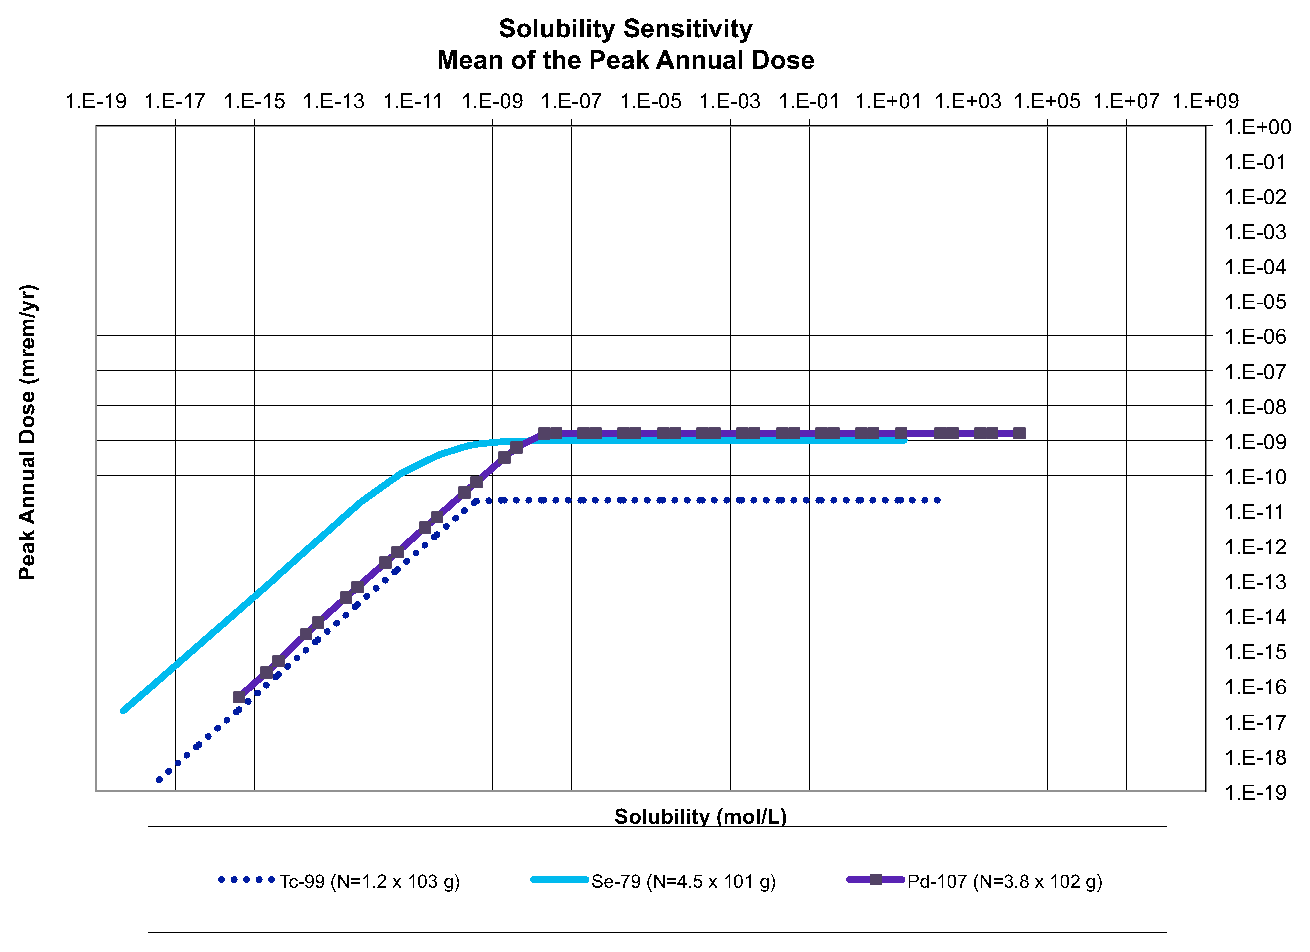
\includegraphics[width=0.7\linewidth]{./chapters/nuclide_sensitivity/clay/Solubility/Solubility_Summary_Sol.eps}
\caption{Solubility limit sensitivity. The peak annual dose due to an inventory, 
$N$, of each isotope.}
\label{fig:SolSum}
\end{figure}
\FloatBarrier
